\documentclass{extbook}[14pt]
\usepackage{multicol, enumerate, enumitem, hyperref, color, soul, setspace, parskip, fancyhdr, amssymb, amsthm, amsmath, bbm, latexsym, units, mathtools}
\everymath{\displaystyle}
\usepackage[headsep=0.5cm,headheight=0cm, left=1 in,right= 1 in,top= 1 in,bottom= 1 in]{geometry}
\usepackage{dashrule}  % Package to use the command below to create lines between items
\newcommand{\litem}[1]{\item #1

\rule{\textwidth}{0.4pt}}
\pagestyle{fancy}
\lhead{}
\chead{Answer Key for Progress Quiz 8 Version C}
\rhead{}
\lfoot{4553-3922}
\cfoot{}
\rfoot{Fall 2020}
\begin{document}
\textbf{This key should allow you to understand why you choose the option you did (beyond just getting a question right or wrong). \href{https://xronos.clas.ufl.edu/mac1105spring2020/courseDescriptionAndMisc/Exams/LearningFromResults}{More instructions on how to use this key can be found here}.}

\textbf{If you have a suggestion to make the keys better, \href{https://forms.gle/CZkbZmPbC9XALEE88}{please fill out the short survey here}.}

\textit{Note: This key is auto-generated and may contain issues and/or errors. The keys are reviewed after each exam to ensure grading is done accurately. If there are issues (like duplicate options), they are noted in the offline gradebook. The keys are a work-in-progress to give students as many resources to improve as possible.}

\rule{\textwidth}{0.4pt}

\begin{enumerate}\litem{
Describe the end behavior of the polynomial below.
\[ f(x) = 6(x + 4)^{3}(x - 4)^{4}(x + 9)^{3}(x - 9)^{3} \]

The solution is the graph below, which is option D.
\begin{center}
    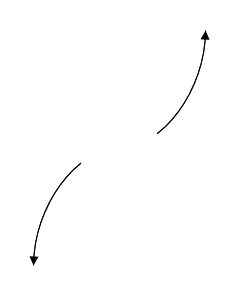
\includegraphics[width=0.3\textwidth]{../Figures/polyEndBehaviorDC.png}
\end{center}\begin{enumerate}[label=\Alph*.]
\begin{multicols}{2}
\item 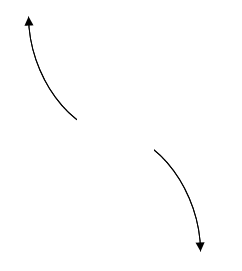
\includegraphics[width = 0.3\textwidth]{../Figures/polyEndBehaviorAC.png}
\item 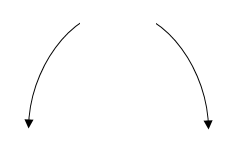
\includegraphics[width = 0.3\textwidth]{../Figures/polyEndBehaviorBC.png}
\item 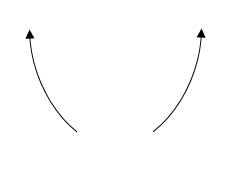
\includegraphics[width = 0.3\textwidth]{../Figures/polyEndBehaviorCC.png}
\item 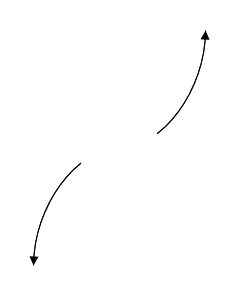
\includegraphics[width = 0.3\textwidth]{../Figures/polyEndBehaviorDC.png}
\end{multicols}\item None of the above.\end{enumerate}
\textbf{General Comment:} Remember that end behavior is determined by the leading coefficient AND whether the \textbf{sum} of the multiplicities is positive or negative.
}
\litem{
Construct the lowest-degree polynomial given the zeros below. Then, choose the intervals that contain the coefficients of the polynomial in the form $ax^3+bx^2+cx+d$.
\[ \frac{-3}{2}, \frac{1}{5}, \text{ and } 6 \]

The solution is \( 10x^{3} -47 x^{2} -81 x + 18 \), which is option C.\begin{enumerate}[label=\Alph*.]
\item \( a \in [6, 11], b \in [47, 50], c \in [-83, -76], \text{ and } d \in [-21, -15] \)

$10x^{3} +47 x^{2} -81 x -18$, which corresponds to multiplying out $(2x -3)(5x + 1)(x + 6)$.
\item \( a \in [6, 11], b \in [-55, -41], c \in [-83, -76], \text{ and } d \in [-21, -15] \)

$10x^{3} -47 x^{2} -81 x -18$, which corresponds to multiplying everything correctly except the constant term.
\item \( a \in [6, 11], b \in [-55, -41], c \in [-83, -76], \text{ and } d \in [16, 25] \)

* $10x^{3} -47 x^{2} -81 x + 18$, which is the correct option.
\item \( a \in [6, 11], b \in [-74, -70], c \in [75, 80], \text{ and } d \in [16, 25] \)

$10x^{3} -73 x^{2} +75 x + 18$, which corresponds to multiplying out $(2x + 2)(5x + 5)(x -1)$.
\item \( a \in [6, 11], b \in [-80, -75], c \in [101, 114], \text{ and } d \in [-21, -15] \)

$10x^{3} -77 x^{2} +105 x -18$, which corresponds to multiplying out $(2x + 2)(5x -5)(x -1)$.
\end{enumerate}

\textbf{General Comment:} To construct the lowest-degree polynomial, you want to multiply out $(2x + 3)(5x -1)(x -6)$
}
\litem{
Describe the zero behavior of the zero $x = -4$ of the polynomial below.
\[ f(x) = 6(x - 4)^{9}(x + 4)^{12}(x + 8)^{3}(x - 8)^{5} \]

The solution is the graph below, which is option C.
\begin{center}
    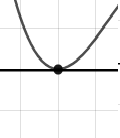
\includegraphics[width=0.3\textwidth]{../Figures/polyZeroBehaviorCopyCC.png}
\end{center}\begin{enumerate}[label=\Alph*.]
\begin{multicols}{2}
\item 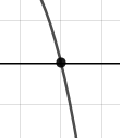
\includegraphics[width = 0.3\textwidth]{../Figures/polyZeroBehaviorCopyAC.png}
\item 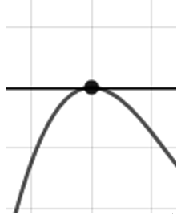
\includegraphics[width = 0.3\textwidth]{../Figures/polyZeroBehaviorCopyBC.png}
\item 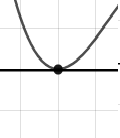
\includegraphics[width = 0.3\textwidth]{../Figures/polyZeroBehaviorCopyCC.png}
\item 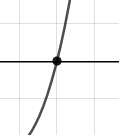
\includegraphics[width = 0.3\textwidth]{../Figures/polyZeroBehaviorCopyDC.png}
\end{multicols}\item None of the above.\end{enumerate}
\textbf{General Comment:} You will need to sketch the entire graph, then zoom in on the zero the question asks about.
}
\litem{
Construct the lowest-degree polynomial given the zeros below. Then, choose the intervals that contain the coefficients of the polynomial in the form $x^3+bx^2+cx+d$.
\[ 5 - 2 i \text{ and } 3 \]

The solution is \( x^{3} -13 x^{2} +59 x -87 \), which is option A.\begin{enumerate}[label=\Alph*.]
\item \( b \in [-16, -12], c \in [59, 62], \text{ and } d \in [-89, -75] \)

* $x^{3} -13 x^{2} +59 x -87$, which is the correct option.
\item \( b \in [-3, 6], c \in [-13, -5], \text{ and } d \in [14, 20] \)

$x^{3} + x^{2} -8 x + 15$, which corresponds to multiplying out $(x -5)(x -3)$.
\item \( b \in [-3, 6], c \in [-4, 0], \text{ and } d \in [-9, 1] \)

$x^{3} + x^{2} -x -6$, which corresponds to multiplying out $(x + 2)(x -3)$.
\item \( b \in [10, 20], c \in [59, 62], \text{ and } d \in [84, 92] \)

$x^{3} +13 x^{2} +59 x + 87$, which corresponds to multiplying out $(x-(5 - 2 i))(x-(5 + 2 i))(x + 3)$.
\item \( \text{None of the above.} \)

This corresponds to making an unanticipated error or not understanding how to use nonreal complex numbers to create the lowest-degree polynomial. If you chose this and are not sure what you did wrong, please contact the coordinator for help.
\end{enumerate}

\textbf{General Comment:} Remember that the conjugate of $a+bi$ is $a-bi$. Since these zeros always come in pairs, we need to multiply out $(x-(5 - 2 i))(x-(5 + 2 i))(x-(3))$.
}
\litem{
Which of the following equations \textit{could} be of the graph presented below?

\begin{center}
    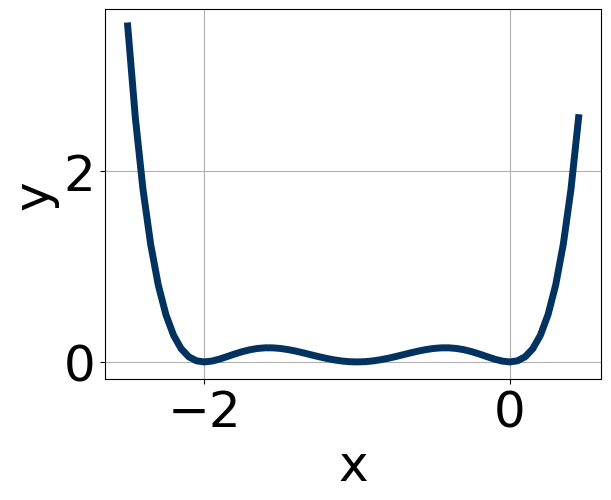
\includegraphics[width=0.5\textwidth]{../Figures/polyGraphToFunctionCopyC.png}
\end{center}




The solution is \( 10x^{4} (x - 1)^{8} (x - 2)^{9} \), which is option B.\begin{enumerate}[label=\Alph*.]
\item \( 10x^{4} (x - 1)^{11} (x - 2)^{5} \)

The factor $(x - 1)$ should have an even power.
\item \( 10x^{4} (x - 1)^{8} (x - 2)^{9} \)

* This is the correct option.
\item \( -6x^{10} (x - 1)^{6} (x - 2)^{6} \)

The factor $(x - 2)$ should have an odd power and the leading coefficient should be the opposite sign.
\item \( -16x^{6} (x - 1)^{10} (x - 2)^{7} \)

This corresponds to the leading coefficient being the opposite value than it should be.
\item \( 10x^{10} (x - 1)^{7} (x - 2)^{4} \)

The factor $(x - 1)$ should have an even power and the factor $(x - 2)$ should have an odd power.
\end{enumerate}

\textbf{General Comment:} General Comments: Draw the x-axis to determine which zeros are touching (and so have even multiplicity) or cross (and have odd multiplicity).
}
\litem{
Describe the zero behavior of the zero $x = 5$ of the polynomial below.
\[ f(x) = 6(x - 5)^{8}(x + 5)^{9}(x - 9)^{2}(x + 9)^{6} \]

The solution is the graph below, which is option C.
\begin{center}
    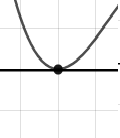
\includegraphics[width=0.3\textwidth]{../Figures/polyZeroBehaviorCC.png}
\end{center}\begin{enumerate}[label=\Alph*.]
\begin{multicols}{2}
\item 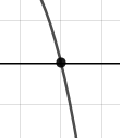
\includegraphics[width = 0.3\textwidth]{../Figures/polyZeroBehaviorAC.png}
\item 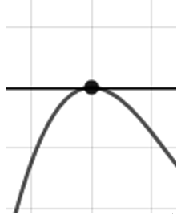
\includegraphics[width = 0.3\textwidth]{../Figures/polyZeroBehaviorBC.png}
\item 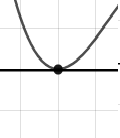
\includegraphics[width = 0.3\textwidth]{../Figures/polyZeroBehaviorCC.png}
\item 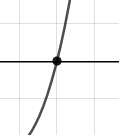
\includegraphics[width = 0.3\textwidth]{../Figures/polyZeroBehaviorDC.png}
\end{multicols}\item None of the above.\end{enumerate}
\textbf{General Comment:} You will need to sketch the entire graph, then zoom in on the zero the question asks about.
}
\litem{
Describe the end behavior of the polynomial below.
\[ f(x) = -9(x - 9)^{3}(x + 9)^{4}(x - 8)^{5}(x + 8)^{6} \]

The solution is the graph below, which is option B.
\begin{center}
    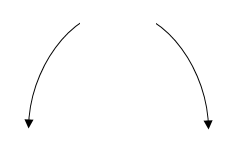
\includegraphics[width=0.3\textwidth]{../Figures/polyEndBehaviorCopyBC.png}
\end{center}\begin{enumerate}[label=\Alph*.]
\begin{multicols}{2}
\item 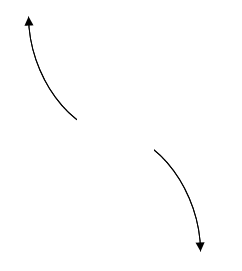
\includegraphics[width = 0.3\textwidth]{../Figures/polyEndBehaviorCopyAC.png}
\item 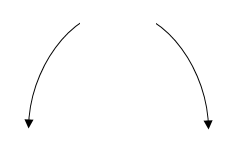
\includegraphics[width = 0.3\textwidth]{../Figures/polyEndBehaviorCopyBC.png}
\item 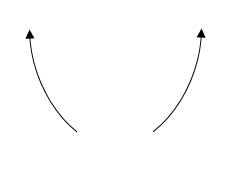
\includegraphics[width = 0.3\textwidth]{../Figures/polyEndBehaviorCopyCC.png}
\item 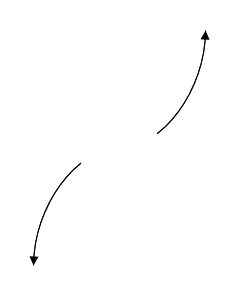
\includegraphics[width = 0.3\textwidth]{../Figures/polyEndBehaviorCopyDC.png}
\end{multicols}\item None of the above.\end{enumerate}
\textbf{General Comment:} Remember that end behavior is determined by the leading coefficient AND whether the \textbf{sum} of the multiplicities is positive or negative.
}
\litem{
Construct the lowest-degree polynomial given the zeros below. Then, choose the intervals that contain the coefficients of the polynomial in the form $x^3+bx^2+cx+d$.
\[ -2 - 4 i \text{ and } -4 \]

The solution is \( x^{3} +8 x^{2} +36 x + 80 \), which is option A.\begin{enumerate}[label=\Alph*.]
\item \( b \in [7, 12], c \in [33.6, 38.7], \text{ and } d \in [78, 88] \)

* $x^{3} +8 x^{2} +36 x + 80$, which is the correct option.
\item \( b \in [-8, -3], c \in [33.6, 38.7], \text{ and } d \in [-82, -75] \)

$x^{3} -8 x^{2} +36 x -80$, which corresponds to multiplying out $(x-(-2 - 4 i))(x-(-2 + 4 i))(x -4)$.
\item \( b \in [-2, 6], c \in [4.5, 7.9], \text{ and } d \in [3, 9] \)

$x^{3} + x^{2} +6 x + 8$, which corresponds to multiplying out $(x + 2)(x + 4)$.
\item \( b \in [-2, 6], c \in [6.8, 9.4], \text{ and } d \in [12, 24] \)

$x^{3} + x^{2} +8 x + 16$, which corresponds to multiplying out $(x + 4)(x + 4)$.
\item \( \text{None of the above.} \)

This corresponds to making an unanticipated error or not understanding how to use nonreal complex numbers to create the lowest-degree polynomial. If you chose this and are not sure what you did wrong, please contact the coordinator for help.
\end{enumerate}

\textbf{General Comment:} Remember that the conjugate of $a+bi$ is $a-bi$. Since these zeros always come in pairs, we need to multiply out $(x-(-2 - 4 i))(x-(-2 + 4 i))(x-(-4))$.
}
\litem{
Construct the lowest-degree polynomial given the zeros below. Then, choose the intervals that contain the coefficients of the polynomial in the form $ax^3+bx^2+cx+d$.
\[ \frac{7}{5}, \frac{-4}{5}, \text{ and } \frac{1}{2} \]

The solution is \( 50x^{3} -55 x^{2} -41 x + 28 \), which is option D.\begin{enumerate}[label=\Alph*.]
\item \( a \in [50, 51], b \in [-63, -50], c \in [-43, -33], \text{ and } d \in [-32, -26] \)

$50x^{3} -55 x^{2} -41 x -28$, which corresponds to multiplying everything correctly except the constant term.
\item \( a \in [50, 51], b \in [51, 56], c \in [-43, -33], \text{ and } d \in [-32, -26] \)

$50x^{3} +55 x^{2} -41 x -28$, which corresponds to multiplying out $(5x + 7)(5x -4)(2x + 1)$.
\item \( a \in [50, 51], b \in [80, 86], c \in [-2, 3], \text{ and } d \in [-32, -26] \)

$50x^{3} +85 x^{2} +x -28$, which corresponds to multiplying out $(5x + 5)(5x -5)(2x -2)$.
\item \( a \in [50, 51], b \in [-63, -50], c \in [-43, -33], \text{ and } d \in [24, 36] \)

* $50x^{3} -55 x^{2} -41 x + 28$, which is the correct option.
\item \( a \in [50, 51], b \in [4, 8], c \in [-73, -67], \text{ and } d \in [24, 36] \)

$50x^{3} +5 x^{2} -71 x + 28$, which corresponds to multiplying out $(5x + 5)(5x + 5)(2x -2)$.
\end{enumerate}

\textbf{General Comment:} To construct the lowest-degree polynomial, you want to multiply out $(5x -7)(5x + 4)(2x -1)$
}
\litem{
Which of the following equations \textit{could} be of the graph presented below?

\begin{center}
    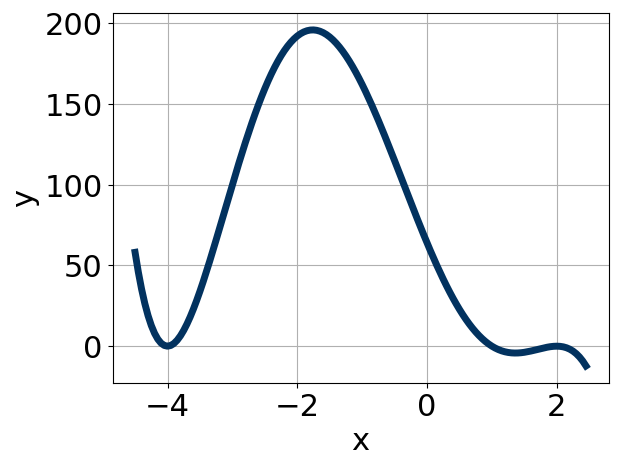
\includegraphics[width=0.5\textwidth]{../Figures/polyGraphToFunctionC.png}
\end{center}




The solution is \( 15x^{7} (x - 1)^{11} (x - 2)^{11} \), which is option A.\begin{enumerate}[label=\Alph*.]
\item \( 15x^{7} (x - 1)^{11} (x - 2)^{11} \)

* This is the correct option.
\item \( -13x^{7} (x - 1)^{9} (x - 2)^{7} \)

This corresponds to the leading coefficient being the opposite value than it should be.
\item \( 19x^{7} (x - 1)^{8} (x - 2)^{6} \)

The factors $1$ and $2$ have have been odd power.
\item \( -15x^{5} (x - 1)^{8} (x - 2)^{7} \)

The factor $(x - 1)$ should have an odd power and the leading coefficient should be the opposite sign.
\item \( 7x^{11} (x - 1)^{6} (x - 2)^{9} \)

The factor $1$ should have been an odd power.
\end{enumerate}

\textbf{General Comment:} General Comments: Draw the x-axis to determine which zeros are touching (and so have even multiplicity) or cross (and have odd multiplicity).
}
\end{enumerate}

\end{document}